\documentclass[10pt, xcolor=table]{beamer}

\setbeamertemplate{note page}[default]
%\setbeameroption{hide notes}
\setbeameroption{show notes}
\setbeamerfont{footnote}{size=\tiny}

\usetheme[progressbar=frametitle]{metropolis}
\usepackage{appendixnumberbeamer}

\usepackage{booktabs}
\usepackage[scale=2]{ccicons}

\usepackage{pgfplots}
\usepgfplotslibrary{dateplot}
\usepackage{multicol}
\setlength{\columnsep}{1.5cm}
\usepackage{multirow}

\usepackage{hyperref}
%\usepackage{animate}
\usepackage{lmodern}
\usepackage[T1]{fontenc}
\usepackage{mathtools}
\usepackage{graphicx}
\usepackage[font=scriptsize]{caption}
\usepackage{tikz}
\usepackage{stackengine}
\usepackage{array}
\usetikzlibrary{positioning}
\usepackage{tabularx}
\usepackage{tabulary}
%\hypersetup{
%    colorlinks=true,
%    linktoc=none,
%    linkcolor=blue,
%    urlcolor=blue
%}

\usepackage[math]{cellspace}
\cellspacetoplimit 2pt
\cellspacebottomlimit 2pt


%\definecolor{set1}{RGB}{228, 26, 28}
%\definecolor{set2}{RGB}{77, 175, 74}
%\definecolor{set3}{RGB}{255, 127, 0}
%\definecolor{set4}{RGB}{166, 86, 40}
%\definecolor{set5}{RGB}{153, 153, 153}

\usepackage{xspace}
\newcommand{\themename}{\textbf{\textsc{metropolis}}\xspace}

\newcommand\Fontvi{\fontsize{8}{9}\selectfont}
\newcommand\Fontvr{\fontsize{6}{7}\selectfont}

\setbeamerfont{parent A}{size=\small}

\DeclarePairedDelimiter\abs{\lvert}{\rvert}%
\DeclarePairedDelimiter\norm{\lVert}{\rVert}%
\makeatletter
\let\oldabs\abs
\def\abs{\@ifstar{\oldabs}{\oldabs*}}
\let\oldnorm\norm
\def\norm{\@ifstar{\oldnorm}{\oldnorm*}}
\makeatother
\newcommand*{\Value}{\frac{1}{2}x^2}%

\newcommand{\floatfootnote}[1]{\ifx\[$\else\footnote{#1}\fi}
\newcommand{\floatfootnotes}[1]{\ifx\[$\else\footnote{#1}\fi}



\title{Digital Transformation of Healthcare}
\subtitle{Ethics in Modeling}
% \date{\today}
\date{}
\author{Michoel Snow, M.D. Ph.D., Glen Ferguson, Ph.D.}
\institute{Center for Health Data Innovations}
% \titlegraphic{\hfill\includegraphics[height=1.5cm]{logo.pdf}}

\begin{document}

\maketitle


\begin{frame}{Ethics in Modeling}
	After this lecture students will be able to 
	\begin{itemize}
		\item Define the costs associated with an intervention
		\item Differentiate between direct and indirect costs 
		\item Locate estimates for direct and indirect costs
		\item Discuss Markov Chain Monte Carlo for modeling costs
	\end{itemize}
\end{frame}


\begin{frame}{Bioinformatics Pipeline}
	\begin{center}
		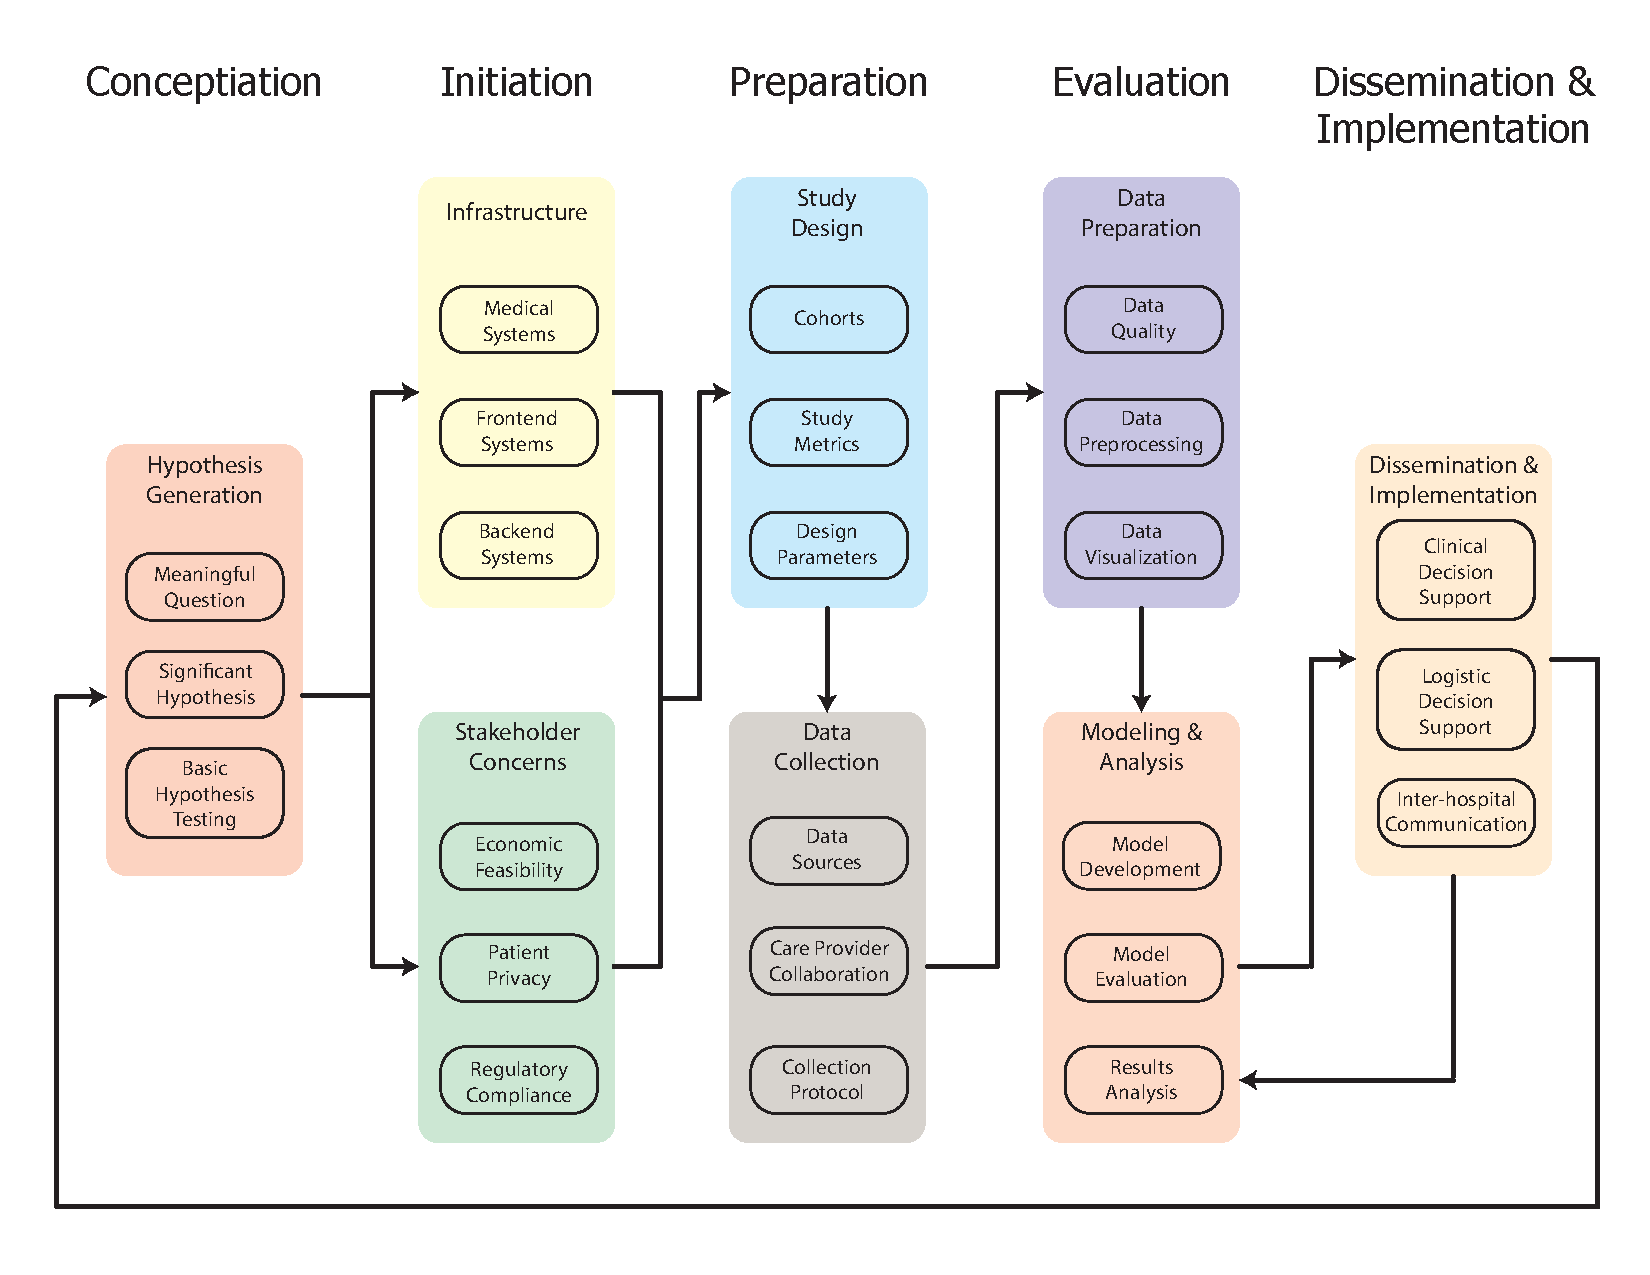
\includegraphics[width=0.9\textwidth]{images/informatics_pipeline.pdf}	
	\end{center}
\end{frame}


\begin{frame}{Economic Valuation}
	\begin{center}
		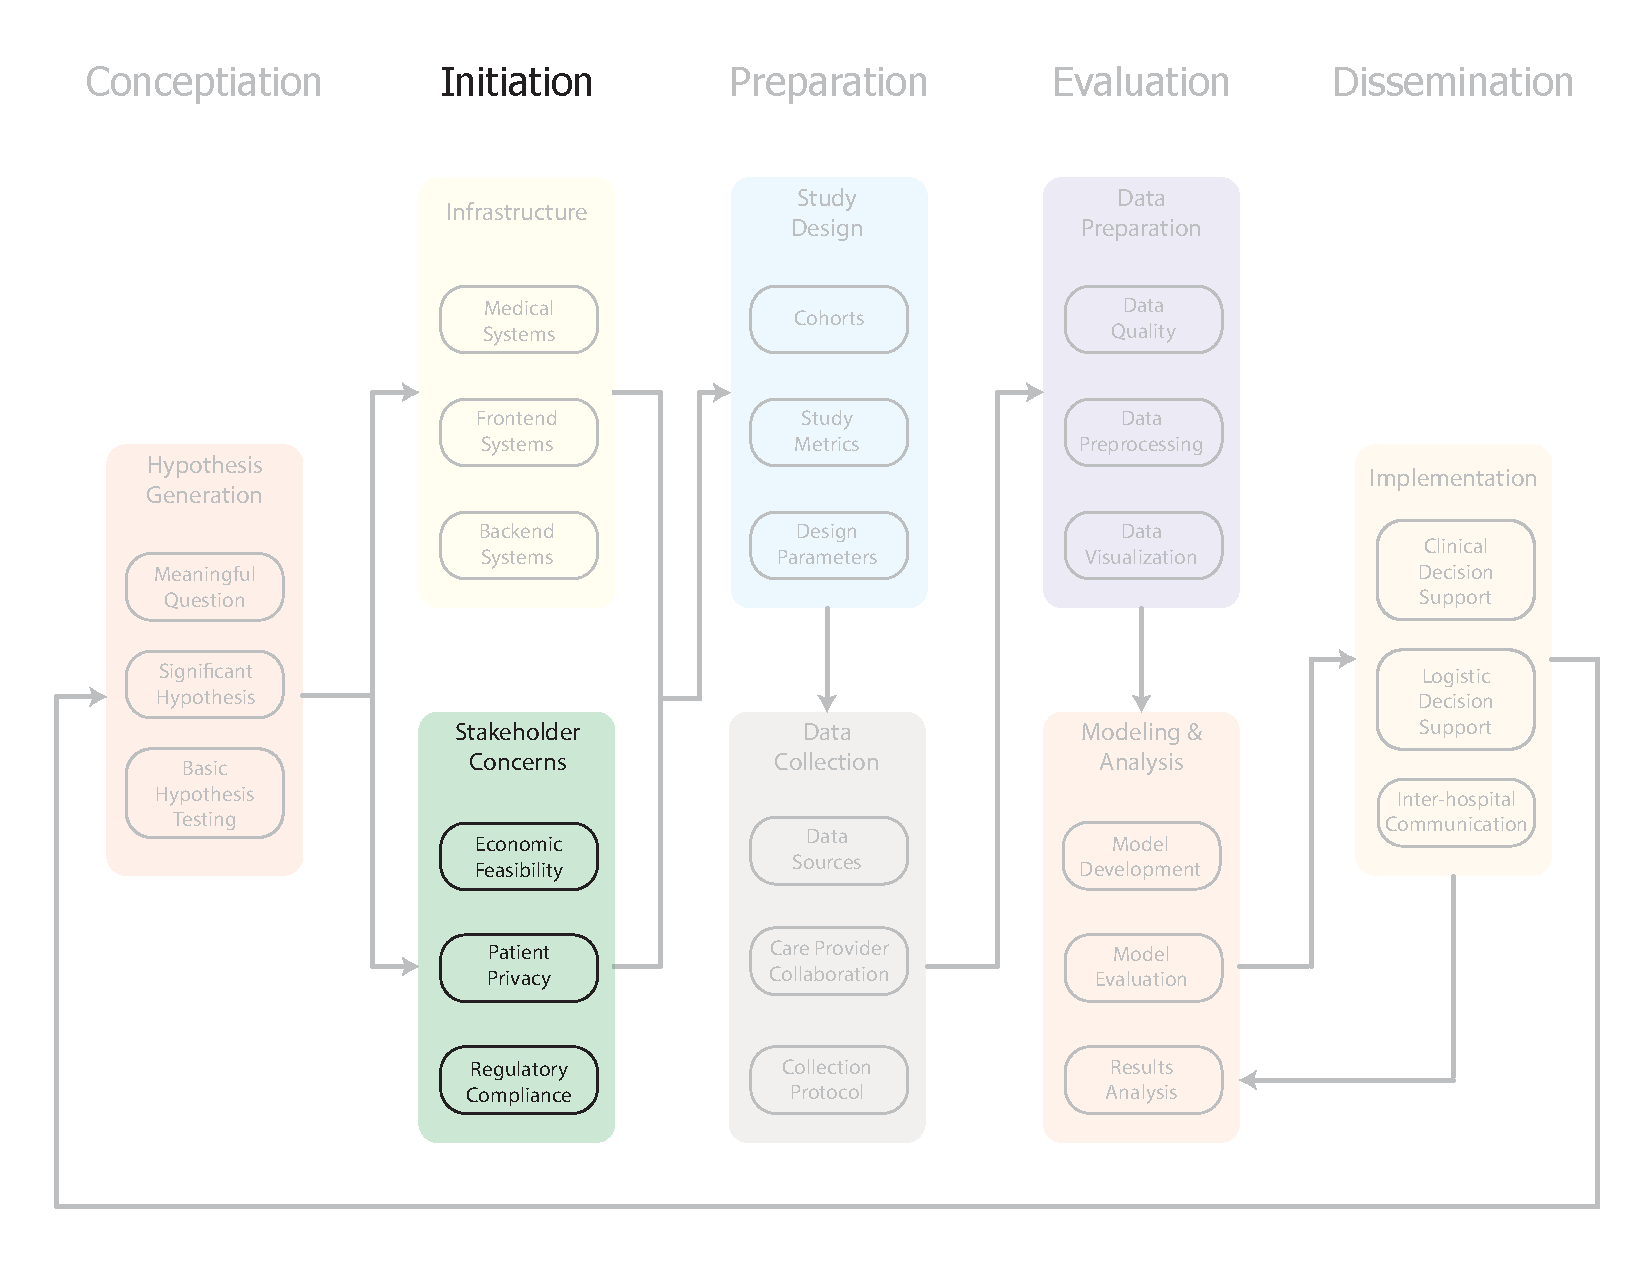
\includegraphics[width=0.9\textwidth]{images/informatics_pipeline_model_ethics.pdf}	
	\end{center}
\end{frame}


\begin{frame}{Case 1\footnote{https://www.propublica.org/article/machine-bias-risk-assessments-in-criminal-sentencing}}
	\begin{itemize}
		\item Risk assessments are used to inform decisions about who can be set free at every stage of the criminal justice system, from assigning bond amounts to even more fundamental decisions about defendants' freedom. 
		\item ProPublica obtained the risk scores assigned to more than 7,000 people arrested in Broward County, Florida, in 2013 and 2014 
		\item The formula was particularly likely to falsely flag black defendants as future criminals, wrongly labeling them this way at almost twice the rate as white defendants.
		\item White defendants were mislabeled as low risk more often than black defendants.
		\item Is this an ethical model?
	\end{itemize}
\end{frame}

\begin{frame}{Case 2}
	\begin{itemize}
		\item You are tasked with developing a protocol for all patients diagnosed with and begin treated for pneumonia.
		\item You decide to use all previous cases where patients where treated for pneumonia to build your neural network, with the inputs being the state of the patients at the beginning of the day and the outputs being the state of the patients at the end of the day?
		\item Are there any ethical concerns with this method of model building?
		\item How can you mitigate ethical issues before they arise?
	\end{itemize}
\end{frame}

\note{
	\scriptsize
	\begin{itemize}
		\item Ethical concerns
		\begin{itemize}
			\scriptsize
			\item Bias - are people being treated differently due to race, ability to pay without any evidence that there are improved outcomes 
			\item Negative outcomes - this model does not weight any outcome better or worse than any other, just uses what has been done before, e.g., if there is a novel treatment that does better than the standard protocol but has only been used in the past year, then it would be suppressed in this model			
		\end{itemize}
		\item Does a model need to be explainable to be ethical
	\end{itemize}

}

\begin{frame}{Patient Privacy and Data Anonymization}
	\begin{itemize}
		\item How Privacy is a fundamental right of patients, but how does that appear when dealing with models.
		\item Does all patient data need to be anonymized before feeding it into the model?
		\item Are there any negatives of feeding in anonymized data into a model?
		\item Where does patient consent fit in the era of big data?
	\end{itemize}
\end{frame}





\end{document}